\documentclass[12pt]{article}

\usepackage[spanish]{babel}
\usepackage{hyperref}
\usepackage{graphicx}
\usepackage{listings}
\usepackage{color}
\usepackage{multicol}
\usepackage{amssymb}
\usepackage{enumitem}
\usepackage{here}
\usepackage{dsfont}
\usepackage{amsmath}
\usepackage{tipa}
\usepackage{float}
\spanishdecimal{.}

\title{Matemáticas para las Ciencias Aplicadas I}
\title{
	Tercera Lista de Problemas \\
	\textbf{Tercera  Parte} \\
	\vspace{1ex}
	\large Matemáticas para las Ciencias Aplicadas I \\
	Facultad de Ciencias, UNAM}

\date{\today}

\author{Flores Morán Julieta Melina \\ Zarco Romero José Antonio}

\begin{document}

\maketitle

%% De la sección 4.4: ejercicios 48 y 53
%% De la sección 4.5: ejercicios 14, 47, 64 y 65
%% De la sección 4.6: ejercicios 24 y 40
%% De la sección 4.7: ejercicios 18 y 34

%%  -----------------------------------------------------------------------------------------------------------------------------------------------------------------------------------------------------------------------------
\section{Sección 4.4 \\ Máximos Y Mínimos Absolutos}
% 48 -------------------------------------------------------------------------------------------------------------
\subsection{Ejercicio 48} name \\

Una forma de demostrar que $f(x) \leq g(x)$ para todo $x$ en un intervalo dado es demostrar que $0 \leq g(x)-f(x)$ para todo $x$ en el intervalo; y una forma de demostrar esta última desigualdad es demostrar que el valor mínimo absoluto de $g(x)-f(x)$ en el intervalo no es negativo. Utilice esta idea para demostrar las desigualdades en estos ejercicios.

Demuestre que $\cos{x} \geq 1-(x^2 /2)$ para todo $x$ en el intervalo $[0, 2\pi]$.

% 53 -------------------------------------------------------------------------------------------------------------
\subsection{Ejercicio 53} name \\

Supongamos que las ecuaciones de movimiento de un avión de papel durante los primeros 12 segundos de vuelo son
\begin{align*}
  x=t-2\sin{t} && y=2-2\cos{t} && (0\leq t\leq 12)
\end{align*}
¿Cuáles son los puntos más alto y más bajo de la trayectoria, y cuándo está el avión en esos puntos?


%%  -----------------------------------------------------------------------------------------------------------------------------------------------------------------------------------------------------------------------------
\section{Sección 4.5 \\ Problemas De Máximos Y Mínimos Aplicados}
% 14 -------------------------------------------------------------------------------------------------------------
\subsection{Ejercicio 14} name \\

Un alambre de 12 pulgadas de largo se puede doblar en un círculo, doblar en un cuadrado o cortar en dos pedazos para formar un círculo y un cuadrado. ¿Cuánto alambre se debe usar para el círculo si el área total encerrada por las figuras debe ser (a) un máximo (b) un mínimo?

% 47 -------------------------------------------------------------------------------------------------------------
\subsection{Ejercicio 47} name \\

Un trapezoide está inscrito en un semicírculo de radio 2 de modo que un lado está a lo largo del diámetro (Figura Ex-47). Encuentra el área máxima posible para el trapezoide. [\textit{Sugerencia}: Exprese el área del trapezoide en términos de $\theta$.]
\begin{figure}[H]
\centering
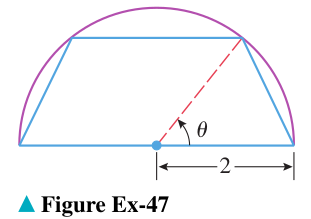
\includegraphics[width=0.4\textwidth]{../img/img_Lista3/3_47.png}
\end{figure}

% 64 -------------------------------------------------------------------------------------------------------------
\subsection{Ejercicio 64} name \\

\textit{\textbf{El principio de Fermat}} en óptica establece que la luz que viaja de un punto a otro sigue aquel camino cuyo tiempo total de viaje es mínimo. En un medio uniforme, los caminos de ``tiempo mínimo'' y ``distancia más corta'' resultan ser los mismos, de modo que la luz, si no hay obstáculos, viaja en línea recta. Supongamos que tenemos una fuente de luz, un espejo plano y un observador en un medio uniforme. Si un rayo de luz sale de la fuente, rebota en el espejo y viaja hasta el observador, entonces su trayectoria constará de dos segmentos de línea, como se muestra en la Figura Ex-64. Según el principio de Fermat, el camino será tal que el tiempo total de viaje $t$ sea mínimo o, dado que el medio es uniforme, el camino será tal que la distancia total recorrida de $A$ a $P$ y a $B$ sea lo más pequeña posible. Suponiendo que el mínimo ocurre cuando $dt/dx = 0$, demuestre que el rayo de luz incidirá en el espejo en el punto $P$ donde el ``ángulo de incidencia'' $\theta_1$ es igual al ``ángulo de reflexión'' $\theta_2$.
\begin{figure}[H]
\centering
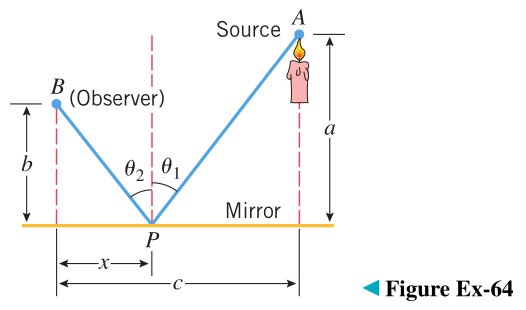
\includegraphics[width=0.7\textwidth]{../img/img_Lista3/3_64.png}
\end{figure}

% 65 -------------------------------------------------------------------------------------------------------------
\subsection{Ejercicio 65} name \\

El principio de Fermat (Ejercicio 64) también explica por qué los rayos de luz que viajan entre el aire y el agua se curvan (refracción). Imagine que tenemos dos medios uniformes (como aire y agua) y un rayo de luz que viaja desde una fuente $A$ en un medio hasta un observador $B$ en el otro medio (Figura Ex-65). Se sabe que la luz viaja a una velocidad constante en un medio uniforme, pero más lenta en un medio denso (como el agua) que en un medio fino (como el aire). En consecuencia, el camino de menor tiempo de A a B no es necesariamente una línea recta, sino más bien un camino de línea discontinua de $A$ a $P$ a $B$ que permite a la luz aprovechar al máximo su mayor velocidad a través del medio delgado. \textit{\textbf{La ley de refracción de Snell}} establece que la trayectoria del rayo de luz será tal que
\[
\frac{\sin{\theta_1}}{v_1}=\frac{\sin{\theta_2}}{v_2}
\]
donde $v_1$ es la velocidad de la luz en el primer medio, $v_2$ es la velocidad de la luz en el segundo medio y $\theta_1$ y $\theta_2$ son los ángulos que se muestran en la figura Ex-65. Demuestre que esto se deriva del supuesto de que la trayectoria del tiempo mínimo ocurre cuando $dt /dx = 0$.
\begin{figure}[H]
\centering
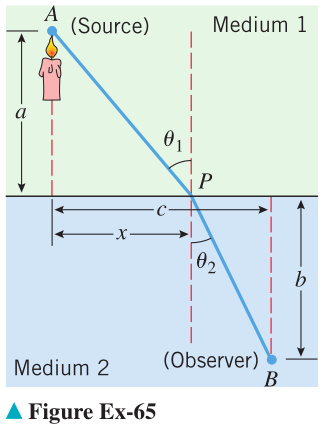
\includegraphics[width=0.4\textwidth]{../img/img_Lista3/3_65.png}
\end{figure}

%%  -----------------------------------------------------------------------------------------------------------------------------------------------------------------------------------------------------------------------------
\section{Sección 4.6 \\ Movimiento Rectilíneo}
% 24 -------------------------------------------------------------------------------------------------------------
\subsection{Ejercicio 24} name \\

Sea $s(t) = t /e^t$ la función de posición de una partícula que se mueve a lo largo de una línea de coordenadas, donde $s$ está en metros y $t$ está en segundos. Utilice una utilidad gráfica para generar las gráficas de $s(t)$, $v(t)$ y $a(t)$ para $t \geq 0$, y utilice esas gráficas cuando sea necesario.
\begin{enumerate}[label=(\alph*)]
\item Utilice la gráfica apropiada para hacer una estimación aproximada del momento en que la partícula invierte por primera vez la dirección de su movimiento; y luego encuentre la hora exacta.
\item Encuentre la posición exacta de la partícula cuando invierte por primera vez la dirección de su movimiento.
\item Utilice las gráficas apropiadas para hacer una estimación aproximada de los intervalos de tiempo en los que la partícula se acelera y en los que se desacelera; y luego encuentre esos intervalos de tiempo exactamente.
\end{enumerate}
    
% 40 -------------------------------------------------------------------------------------------------------------
\subsection{Ejercicio 40} name \\

Sean $s_A = 15t^2 + 10t + 20$ y $s_B = 5t^2 + 40t, t \geq 0$, las funciones de posición de los automóviles $A$ y $B$ que se mueven a lo largo de carriles rectos paralelos de una carretera.

\begin{enumerate}[label=(\alph*)]
\item ¿A qué distancia está el automóvil $A$ por delante del automóvil $B$ cuando $t = 0$?
\item ¿En qué instantes de tiempo están los autos uno al lado del otro?
\item ¿En qué instante de tiempo tienen la misma velocidad? ¿Qué coche va delante en este instante?
\end{enumerate}

%%  -----------------------------------------------------------------------------------------------------------------------------------------------------------------------------------------------------------------------------
\section{Sección 4.7 \\ Método De Newton}
% 18 -------------------------------------------------------------------------------------------------------------
\subsection{Ejercicio 18} name \\

Utilice una utilidad gráfica para determinar el número de veces que se cruzan las curvas; y luego aplique el método de Newton, cuando sea necesario, para aproximar las coordenadas x de todas las intersecciones.
\[
y=\frac{1}{8}x^3-1 \qquad \text{ y } \qquad y=\cos{x}-2
\]

% 34 -------------------------------------------------------------------------------------------------------------
\subsection{Ejercicio 34} name \\

Un \textit{\textbf{segmento}} de círculo es la región encerrada por un arco y su cuerda (Figura Ex-34). Si $r$ es el radio del círculo y $\theta$ el ángulo subtendido en el centro del círculo, entonces se puede demostrar que el área $A$ del segmento es $A = \frac{1}{2} r^2 (\theta - \sin{\theta})$, donde $\theta$ está en radianes. Encuentre el valor de $\theta$ para el cual el área del segmento es un cuarto del área del círculo. Calcula $\theta$ al grado más cercano.

\begin{figure}[H]
\centering
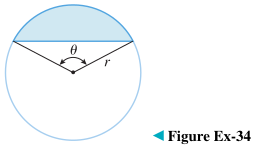
\includegraphics[width=0.5\textwidth]{../img/img_Lista3/3_34.png}
\end{figure}

\end{document}
